%Dokumentklasse

%draft als optionohne bilder für bessere performance
%\documentclass[a4paper,12pt,]{scrreprt}

%normal mit Bildern
\documentclass[
a4paper,
11pt,
draft=True]
{scrartcl}

%Section als Chapter
\RedeclareSectionCommand[%
%beforeskip = -1sp plus -1sp minus -1sp,% kleinster negativer Wert, um den Absatzeinzug nach der Überschrift zu verhindern.
afterskip = 1.5 \baselineskip plus -1sp minus 1sp,
font = \Huge,
]{section}

\usepackage[left= 3cm,right = 3cm, bottom = 3cm,top = 3cm]{geometry}
%\usepackage[onehalfspacing]{setspace}

% ============= Packages =============
% Dokumentinformationen
\usepackage[
pdftitle={Praktikum - Umwelttechnik},
pdfsubject={},
pdfauthor={Roman-Luca Zank},
pdfkeywords={},	
%Links nicht einrahmen
hidelinks
]{hyperref}

%nur Text zum prüfen des Umfangs

% Standard Packages
%\usepackage[bottom]{footmisc}
\usepackage[utf8]{inputenc}
\usepackage[ngerman]{babel}

\usepackage[T1]{fontenc}
%\usepackage{helvet}

%\renewcommand{\familydefault}{\sfdefault}

\usepackage{graphicx}
\graphicspath{{img/}}
\usepackage{mhchem}
\usepackage{fancyhdr}
\usepackage{lmodern}
\usepackage{color}
\usepackage[bottom]{footmisc}
\usepackage{setspace}\usepackage{threeparttable}
%==================================================================
%\begin{threeparttable} 
%	\begin{tabular}{|l|c|r|} 
%		\hline 
%		A & B & C \\
%		\hline
%		1 & 2 & 3 \tnote{1} \\
%		\hline
%	\end{tabular} 
%	\begin{tablenotes}\footnotesize 
%		\item[1] Prognose 2003 
%	\end{tablenotes}
%====================================================================
\usepackage{placeins}
\usepackage{booktabs}
\usepackage{caption}
\usepackage[list=true]{subcaption}
\usepackage{longtable}
\usepackage{tikz}
\usepackage{pgfplots}
\usepackage{lastpage}
%\usepackage{ulem}
\usepackage{mathtools}
\usepackage{adjustbox}
\usetikzlibrary{patterns}
\usepackage{pdfpages}

%Einheitenpackage
\usepackage{siunitx}  
\sisetup{	locale = DE, 
	per-mode=fraction,
	inter-unit-product=\ensuremath{\cdot},
	detect-weight = true,
	quotient-mode=fraction
}
%neue Einheiten definieren
\DeclareSIUnit\xyz{xyz}	
\DeclareSIUnit\rpm{rpm}	
\DeclareSIUnit\mws{mWS}	
\DeclareSIUnit\degrees{^\circ}	

%Automatisch cdot statt *
\DeclareMathSymbol{*}{\mathbin}{symbols}{"01}


%Tabelle
\usepackage{tabularx}
\usepackage{tabulary}

%nur letzte Zeile der Gleichung nummerieren
\makeatletter
\def\Let@{\def\\{\notag\math@cr}}
\makeatother

% zusätzliche Schriftzeichen der American Mathematical Society
\usepackage{amsfonts}
\usepackage{amsmath}

%Abkürzungsverzeichnis
\usepackage{acronym}

%kein Abstand bei neuem Kapitel vom Seitenanfang
%\vspace*{2.3\baselineskip} = ORIGINAL
%\renewcommand*{\chapterheadstartvskip}{\vspace*{.0\baselineskip}}

%nicht einrücken nach Absatz
\setlength{\parindent}{0pt}

\urlstyle{same}


% ============= Kopf- und Fußzeile =============
\pagestyle{fancy}
%
\lhead{}
\chead{}
\rhead{}%\slshape }%\leftmark}
%%
\lfoot{}
\cfoot{}
\rfoot[{\thepage\ of \pageref*{LastPage}}]{Seite \thepage\ von \pageref*{LastPage}}
%%
\renewcommand{\headrulewidth}{0pt}
\renewcommand{\footrulewidth}{0pt}
%\renewcommand{\chapterpagestyle}{fancy}

%Fußnotelinie
%\let\footnoterule

%Fußnote mit Klammer
\renewcommand*{\thefootnote}{(\arabic{footnote})}

%Abb. statt Abbildung
\addto\captionsngerman{%
	\renewcommand{\figurename}{Abb.}%
	\renewcommand{\tablename}{Tab.}%
}

% ============= Package Einstellungen & Sonstiges ============= 
%Besondere Trennungen
%\hyphenation{De-zi-mal-tren-nung}
\usepackage[none]{hyphenat}
\hyphenpenalty=5000
\tolerance=5000
\providecommand\phantomsection{}

\usepackage{mathtools}


% ============= Dokumentbeginn =============

\begin{document}
%Seiten ohne Kopf- und Fußzeile sowie Seitenzahl
\pagestyle{empty}

%\begin{center}
\begin{tabular}{p{\textwidth}}


\begin{center}

\includegraphics[scale=0.75]{logos.jpg}\\
\end{center}


\\

\begin{center}
\LARGE{\textsc{
Protokoll \\
Thermische Verfahrenstechnik\\
}}
\end{center}

\\

%\begin{center}
%\large{Fakultät für Muster und Beispiele \\
%der Hochschule Musterhausen \\}
%\end{center}
%
%\\
\begin{center}
	\textbf{\LARGE{Destillation}}\\
	\vspace{5mm}
	%\textbf{\Large{Destillation}}

\end{center}
\begin{center}
%\Large{Bestimmung des Wassergehalt von Flüssigkeiten und Feststoffen (Iodometrie)}
\end{center}

\begin{center}
	\large{Datensatz J}
\end{center}


\\
%\begin{center}
%zur Erlangung des akademischen Grades\\
%Bachelor of Engineering
%\end{center}


%\begin{center}
%vorgelegt von
%\end{center}

\begin{center}
\Large{\textbf{Teilnehmer:}} \\ 
\end{center}
\begin{center}
\large{Roman-Luca Zank \\
	Willy Messerschmidt} \\
\end{center}


\\

\begin{center}
\begin{tabular}{lll}
%\large{\textbf{Protokollführer:}} & & \large{NAME}\\
&&\\
\large{\textbf{Datum der Versuchsdurchführung:}}&& \large{ (Online)}\\
&&\\
\large{\textbf{Abgabedatum:}}&& \large{\today}
\end{tabular}
\end{center}

\\ \\ \\ \\ \\ \\ \\ \\ 
\large{Merseburg den \today}

\end{tabular}
\end{center}


%\include{14_danksagungen}

%\include{15_zusammenfassung}

% Beendet eine Seite und erzwingt auf den nachfolgenden Seiten die Ausgabe aller Gleitobjekte (z.B. Abbildungen), die bislang definiert, aber noch nicht ausgegeben wurden. Dieser Befehl fügt, falls nötig, eine leere Seite ein, sodaß die nächste Seite nach den Gleitobjekten eine ungerade Seitennummer hat. 
\cleardoubleoddpage

% Pagestyle für Titelblatt leer
\pagestyle{empty}

%Seite zählen ab
\setcounter{page}{0}

%Titelblatt
\begin{center}
\begin{tabular}{p{\textwidth}}


\begin{center}

\includegraphics[scale=0.75]{logos.jpg}\\
\end{center}


\\

\begin{center}
\LARGE{\textsc{
Protokoll \\
Thermische Verfahrenstechnik\\
}}
\end{center}

\\

%\begin{center}
%\large{Fakultät für Muster und Beispiele \\
%der Hochschule Musterhausen \\}
%\end{center}
%
%\\
\begin{center}
	\textbf{\LARGE{Destillation}}\\
	\vspace{5mm}
	%\textbf{\Large{Destillation}}

\end{center}
\begin{center}
%\Large{Bestimmung des Wassergehalt von Flüssigkeiten und Feststoffen (Iodometrie)}
\end{center}

\begin{center}
	\large{Datensatz J}
\end{center}


\\
%\begin{center}
%zur Erlangung des akademischen Grades\\
%Bachelor of Engineering
%\end{center}


%\begin{center}
%vorgelegt von
%\end{center}

\begin{center}
\Large{\textbf{Teilnehmer:}} \\ 
\end{center}
\begin{center}
\large{Roman-Luca Zank \\
	Willy Messerschmidt} \\
\end{center}


\\

\begin{center}
\begin{tabular}{lll}
%\large{\textbf{Protokollführer:}} & & \large{NAME}\\
&&\\
\large{\textbf{Datum der Versuchsdurchführung:}}&& \large{ (Online)}\\
&&\\
\large{\textbf{Abgabedatum:}}&& \large{\today}
\end{tabular}
\end{center}

\\ \\ \\ \\ \\ \\ \\ \\ 
\large{Merseburg den \today}

\end{tabular}
\end{center}
 %Prokolle
%\begin{center}
\begin{tabular}{p{\textwidth}}


\begin{center}

\includegraphics[scale=0.75]{img/logos.jpg}\\
\end{center}


\\

\begin{center}
\LARGE{\textsc{
Recherche \\
Rückgewinnung von Ammoniak aus Industrieabwässern\\
}}
\end{center}

%\begin{center}
%\large{Fakultät für Muster und Beispiele \\
%der Hochschule Musterhausen \\}
%\end{center}
%
%\\
 \\
 
\begin{center}
\textbf{\Large{Seminararbeit in Medienrecherche}}
\end{center}

\begin{center}
	\large{im WiSe 2019}
\end{center}
 \\
%\begin{center}
%zur Erlangung des akademischen Grades\\
%Bachelor of Engineering
%\end{center}


\begin{center}
\large{vorgelegt von}
\end{center}
\\


\begin{center}
\Large{\textbf{Roman-Luca Zank}} \\
\end{center}

\begin{center}
3. Semester \\
Chemie- und Umwelttechnik \\
\end{center}


\begin{center}
\begin{tabular}{lll}
	\textbf{E-Mail:} & & romanzank@mail.de\\
	\textbf{Matrikelnummer:} & &25240\\
	\textbf{Adresse:} & &Platz der Bausoldaten 2, Zimmer 224\\
	\textbf{Ort:} & &06217 Merseburg\\
	&& \\
	\textbf{Prüfer:} & & Dr. Frank  Baumann\\
\end{tabular}
\end{center}

\\ \\ \\ \\ \\
\large{Merseburg, \today}

\end{tabular}
\end{center}
 %Seminar-/Abschlussarbeit

% Pagestyle für Rest des Dokuments
\pagestyle{fancy}

%Inhaltsverzeichnis
\tableofcontents
\thispagestyle{empty}

%Inhalt
%
%Verzeichnis aller Bilder
\label{sec:bilder}
\listoffigures
\addcontentsline{toc}{chapter}{Abbildungsverzeichnis}
\thispagestyle{empty}

%Verzeichnis aller Tabellen
\label{sec:tabellen}
\listoftables
\addcontentsline{toc}{chapter}{Tabellenverzeichnis}
\thispagestyle{empty}



%%Abkürzungsverzeichnis
%\setlength{\columnsep}{20pt}
%\twocolumn
%\addchap{Nomenklatur}
%\label{sec:abkurzung}
%\begin{acronym}
%\acro{kf}[$\text{k}_\text{f}$]{Durchlässigkeitsbeiwert}
%\acro{t}{Durchlaufzeit}
%\acro{tm}[$\text{t}_\text{m}$]{Mittlere Durchlaufzeit}
%\acro{V}{Volumen}
%\acro{h}{Höhe der Wassersäule}
%\acro{Q}{Volumenstrom}
%\acro{l}{Durchströmte Länge}
%\acro{A}{Grundfläche}
%\acro{d}{Durchmesser}
%
%\end{acronym}
%\subsubsection{Aufrufen einer Abkürzung}
%\acs{rT}
%\begin{verbatim}
%\acs{Abkürzung}
%\end{verbatim}

%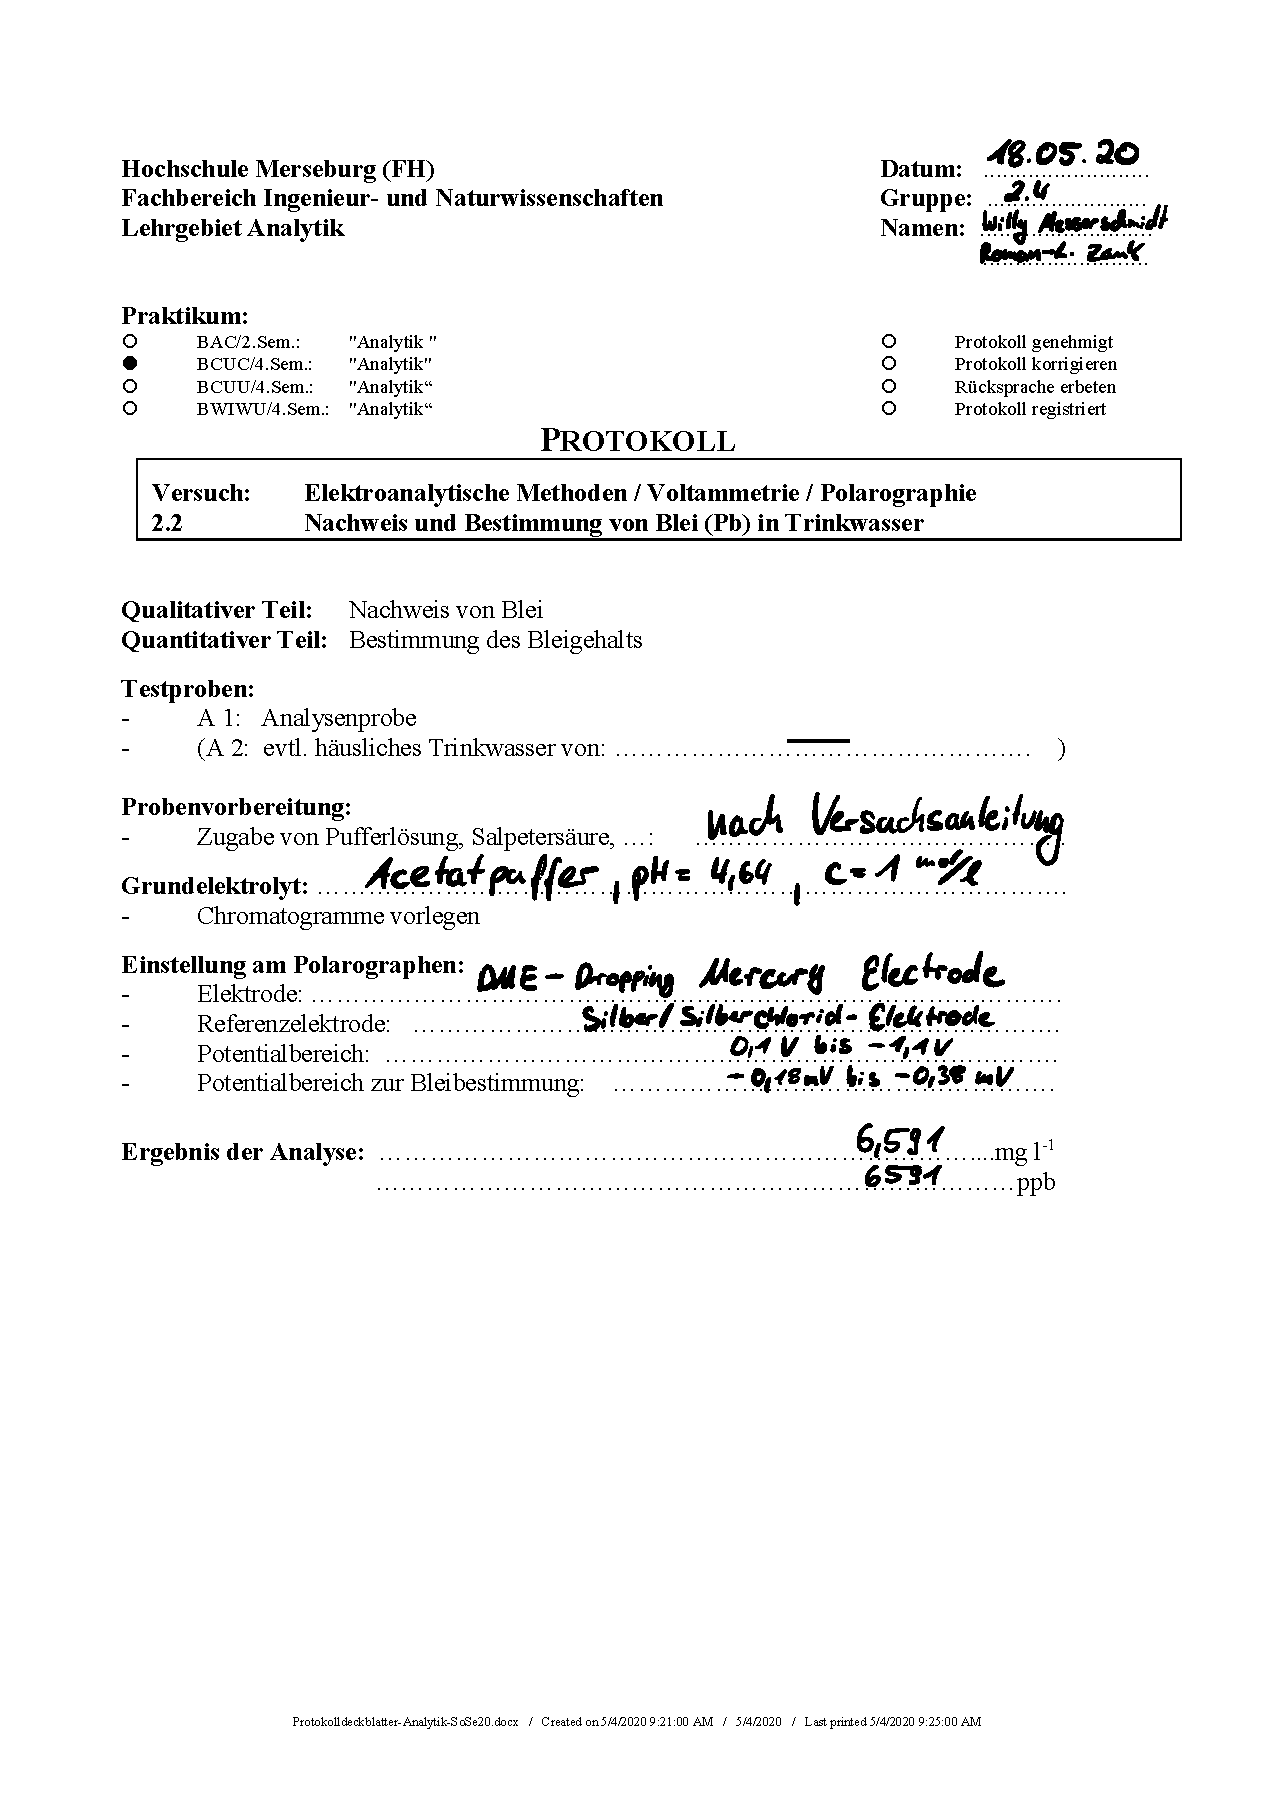
\includepdf[]{Deckblatt}
\pagebreak
\section{Einleitung}
\label{sec:einleitung}
Im Praktikumsversuch wird die Abhängigkeit von Kopf- und Sumpfprodukt-Konzentration vom Rücklaufstrom und der Heizleistung untersucht. Es steht dazu eine Glockenbodenkolonne mit einem Ethanol-Wasser-Gemisch bereit. Die Betriebszustände sollen in McCabe-Thiele-Diagrammen dargestellt werden. Die aus der Stufenkonstruktion bestimmte Anzahl dheoretischer Trennstufen wird hernach mit der wirklichen Anzahl verglichen. Die Anlage wird zudem in stofflicher und energetischer Hinsicht bilanziert.





\section{Theorie}
\label{sec:theorie}

Die Rektifikation als Sonderform der Destillation ist ein Trennverfahren für untereinander mischbare Flüssigkeiten. Der Mischung wird dazu Wärme zugeführt, bis eine teilweise Verdampfung eintritt. Der gewonnene Dampf unterscheidet sich in der Zusammensetzung von der des flüssigen Gemisches. Durch die räumlich getrennte Kondensation dieses Dampfes findet eine Anreicherung einer Komponente im Kondensat statt. Bei der Rektifikation wird diese Anreicherung durch die spezielle Bauform einer Destillationskolonne (in diesem Falle Glockenbodenkolonne) viele Male energiesparend wiederholt.
\newpage
\section{Geräte und Chemikalien}
\label{sec:geraete}

\textbf{Geräte:}
\begin{itemize}
\item Rektifikationsanlage
\item Mettler-Toledo Density Meter DE-40
\item Spritze
\item Bechergläser
\end{itemize}

\vspace*{5mm}

\textbf{Proben/Chemikalien:}
\begin{itemize}
\item Wasser
\item Ethanol

\end{itemize}







\section{Durchführung}
\label{sec:durchfuerung}
Der Versuch wurde nicht selbst durchgeführt. Die nachfolgende grobe Beschreibung des Versuchsablaufes basiert auf einem Videofilm, welcher freundlicher Weise zur Verfügung gestellt wurde. \\
Zu beginn gilt es die Strom und Kühlwasserzufuhr freizugeben. Der Kühlwasserstrom sollte sich zwischen \SI{25}{\liter} und \SI{50}{\liter} betragen. Die Heizung wird zum Hochfahren der Anlage auf 80\% ihrer Leistung engestellt. später kann die Leistung auf 41\% herunter geregelt werden. Die Überwachung der Anlage erfolgt am PC, wo das Programm \emph{Destillation} einen Kernbildschirm erzeugt.
Die Sammelbehälter werden erst einmal geleert. Diese werden wieder freigegeben, wenn sich die Anlage ihren Betriebszustand erreicht hat. Es wird die Ausbildung des thermischen Gleichgewichtes abgewartet. Zum Zeitpunkt der Probennahme wird ein Screenshot am Computer gemacht, Proben an den Sammelbehältern für Sumpf, Feed und Kopfprodukt genommen, und die Füllstände an den Sammelbehältern abgelesen, um daraus den Volumenstrom berechnen zu können. Es ist wichtig die Probennahmestellen vorher zu spülen, weil sich noch alte Mischung darin befindet. Zur Korrektur des Rücklufstroms ist außerdem die Verweilzeit des Magnetventils in der unterren Stellung zu dokumentieren.

Die Flüssigkeitsproben werden im Dichte-Messgerät analysiert.

Die Anlage wird heruntergefahren indem zuerst die Heizung abgeschalten wird. Anschließend wird der Inhalt der Sammelbehälter zurückgepumpt. Schließlich kann auch die Kühlwasserzufuhr und die Stromversorgung abgeschnitten werden.

\newpage
\section{Ergebnisse und Berechnungen}
\label{sec:ergebnisse}
%Tabelle START
\begin{figure}[h!]
	\centering
	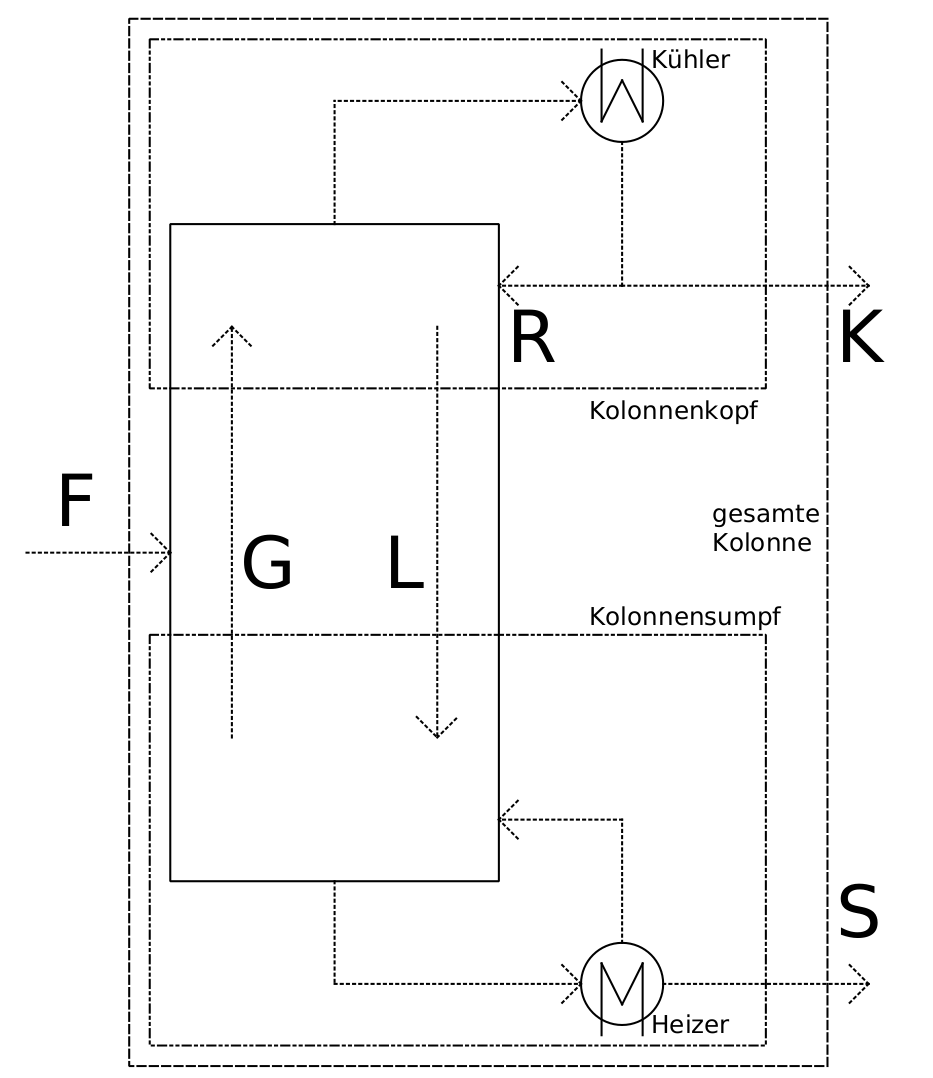
\includegraphics[width=0.7\linewidth]{img/Bilanzraumm}
	\caption{Schematische Abbildung der Rektifikationskolonne zur Darstellung der Bilanzräume}
	\label{fig:Bilanzraumm}
\end{figure}
\FloatBarrier
\subsection{Bilanzen}
\subsubsection{Gesamte Kolonne}

\hspace{5mm}\textbf{Gesamtmolbilanz}\\
\begin{equation}\label{gl:gesamtmolbilanzKOLONNE}
\dot{n}_F=\dot{n}_S+\dot{n}_K
\end{equation}

\hspace{5mm}\textbf{Komponentenbilanz - Ethanol} \\
\begin{equation}\label{gl:komponentenbilanzKOLONNE}
\dot{n}_F*x_{1F}=\dot{n}_S*x_{1F}+\dot{n}_K+x_{1K}
\end{equation}

\hspace{5mm}\textbf{Energiebilanz}\\
\begin{equation}\label{gl:energiebilanzKOLONNE}
\dot{H}_F+Q_{Heiz}=\dot{H}_K+\dot{H}_S+Q_{Kondensator}+Q_{Verlust}
\end{equation}


\subsubsection{Kolonnenkopf}

\hspace{5mm}\textbf{Gesamtmolbilanz}\\
\begin{equation}
\dot{n}_G=\dot{n}_L+\dot{n}_K
\end{equation}

\hspace{5mm}\textbf{Komponentenbilanz - Ethanol} \\
\begin{equation}
\dot{n}_G*y_{1}=\dot{n}_L*x_{1}+\dot{n}_K+x_{1K}
\end{equation}

\hspace{5mm}\textbf{Energiebilanz}\\
\begin{equation}
\dot{H}_G=\dot{H}_K+\dot{H}_L+Q_{Kondensator}+Q_{Verlust}
\end{equation}

\subsection{Berechnung der Zusammensetzung aus der Dichte}

Der Massenanteil an Ethanol der Proben wurde aus den gemessenen Dichten, durch einsetzen in eine Kalibrierfunktion berechnet. 
Die gegebene Kalibrierfunktion ist in Gleichung \eqref{gl:massenanteilausdichte} aufgeführt. 

\begin{equation}\label{gl:massenanteilausdichte}
	\rho=-0,0079826782*(w_1[\%])^2-1,2901290063*(w_1[\%])+998,2
\end{equation}
\subsection{Umrechnung von Massen- in Molenbruch}

Die zuvor erhaltenen Massenanteile werden nun, wie in Gleichung \eqref{gl:massINmol} gezeigt, in die entsprechenden Stoffmengenanteile umgerechnet.
\begin{flalign}\label{gl:massINmol}
	x_i&=\frac{\frac{w_i}{M_i}}{\sum\frac{w_j}{M_j}}\\
			x_1&=\frac{\frac{0,845}{\SI{46,07}{\gram\per\mole}}}{\frac{0,845}{\SI{46,07}{\gram\per\mole}}+\frac{1-0,845}{\SI{18,02}{\gram\per\mole}}}\\
			&=\underline{0,68}
\end{flalign}
\subsection{Berechnung des Molenstromes}

Die Berechnung des Molenstromes der Komponente 1 (Ethanol) an den betrachteten stellen wird analog der Beispielrechnung \eqref{gl:molenstrom} vorgenommen. Dabei werden die gemessene Dichte, der gemessene Volumenstrom, der berechnete Massenanteil und die Molare Masse der betrachteten Komponente eingesetzt.\\
\begin{flalign}\label{gl:molenstrom}
	\dot{n}&=\frac{\rho*\dot{V}*w}{M}\\
\dot{n}_{1K}	&=\frac{\rho_K*\dot{V}_K*w_{1K}}{M_1}\\
	&=\frac{\SI{832,3}{\kilogram\per\cubic\meter}*\SI{0,372}{\liter\per\hour}*0,845}{\SI{46,07}{\gram\per\mole}}\\
	&=\underline{\SI{5,67}{\mole\per\hour}}
\end{flalign}
Der gesamte Molenstrom an einer Stelle wird anschließend unter Zuhilfenahme des Molenbruchs der Komponente ausgerechnet.

\begin{flalign}
	\dot{n}_K&=\frac{\dot{n}_{1K}}{x_{1K}}\\
	&=\frac{\SI{5,67}{\mole\per\hour}}{0,68}\\
	&=\underline{\SI{8,34}{\mole\per\hour}}
\end{flalign}
\subsection{Berechnung des Molenstromes im Sumpf}

Aus den Bilanzgleichungen \eqref{gl:gesamtmolbilanzKOLONNE} und \eqref{gl:komponentenbilanzKOLONNE} ergibt sich ein überbestimmtes Gleichungssystem. Die Berechnung des Molenstromes im Sumpf der Kolonne erfolgt durch Anwendung des Excel-Add-inns \emph{solver}. Der Feed-Molenstrom wird aufgrund der größten Fehleranfälligkeit als veränderliche Größe markiert. Nebenbedingung für die Lösung ist, dass  \eqref{gl:gesamtmolbilanzKOLONNE} und \eqref{gl:komponentenbilanzKOLONNE} den selben wert annehmen. Für die Daten des ersten Versuches folgt ein Sumpf-Molenstrom von \SI{227,27}{\mole\per\hour}. Der Feed-Molenstrom wird durch die Anwendung von ursprünglich \SI{225,39}{\mole\per\hour} auf \SI{235,60}{\mole\per\hour} angehoben. 


\subsection{Rücklaufverhältnis}
Bei einem stationären Betrieb der Rektifikationskolonne im thermischen Gleichgewicht ist auch der Volumenstrom an Kopfprodukt stationär. Daher können für das Rücklaufverhältnis auch die Zeiten eingesetzt werden, in welchen das Magnetventil den jeweiligen Weg freigibt. Dabei wurde die sich auf dem Verschlussstopfen gesammelte Flüssigkeitspfütze berücksichtigt.

\begin{equation}
	\nu=\frac{\dot{R}}{\dot{E}}=\frac{t_{\dot{R}}}{t_{\dot{E}}}=\frac{\SI{11,01}{\second}}{\SI{3,99}{\second}}=\underline{2,76}
\end{equation}

\subsection{McCabe-Thiele-Diagramm}
Nachdem die Ethanolanteile von Kopfprodukt, Feed und Sumpfprodukt als senkrechte Linien in das Gleichgewichtsdiagramm eingetragen sind, kann die Arbeitsgerade des Verstärkungsteils aus dem Punkt $y_o$(vgl.\eqref{gl:yo}) und dem Schnittpunkt von Diagonale und senkrechter auf $x_K$ durch Verbinden der beiden Punkte konstruiert werden. Die Abtriebsgerade folgt aus dem Schnittpunkt der Senkrechten über $x_F$ und der Verstärkungsgerade und dem Schnittpunkt der senkrechten über $x_S$ mit der Diagonalen. Die Stufenkonstruktion erfolgt ausgehend vom Schnittpunkt von Diagonale und senkrechter auf $x_K$, bis zum überschreiten des Schnittpunktes von Diagonale und senkrechter auf $x_S$. Die fertige Stufenkonstruktion ist in Abb. \ref{fig:McCabe} dargestellt. Es ergaben sich 6 theoretische Trennstufen. Diese Anzahl liegt weit unter der wirklichen Bodenzahl von 15. 

\begin{flalign}\label{gl:yo}
	y_o&=\frac{x_K}{\nu+1}\\
	&= \frac{x_K}{\nu+1}=\frac{0,68}{2,76+1}=\underline{0,181}
\end{flalign}
\vspace{-2mm}
\begin{figure}[h!]
	\centering
	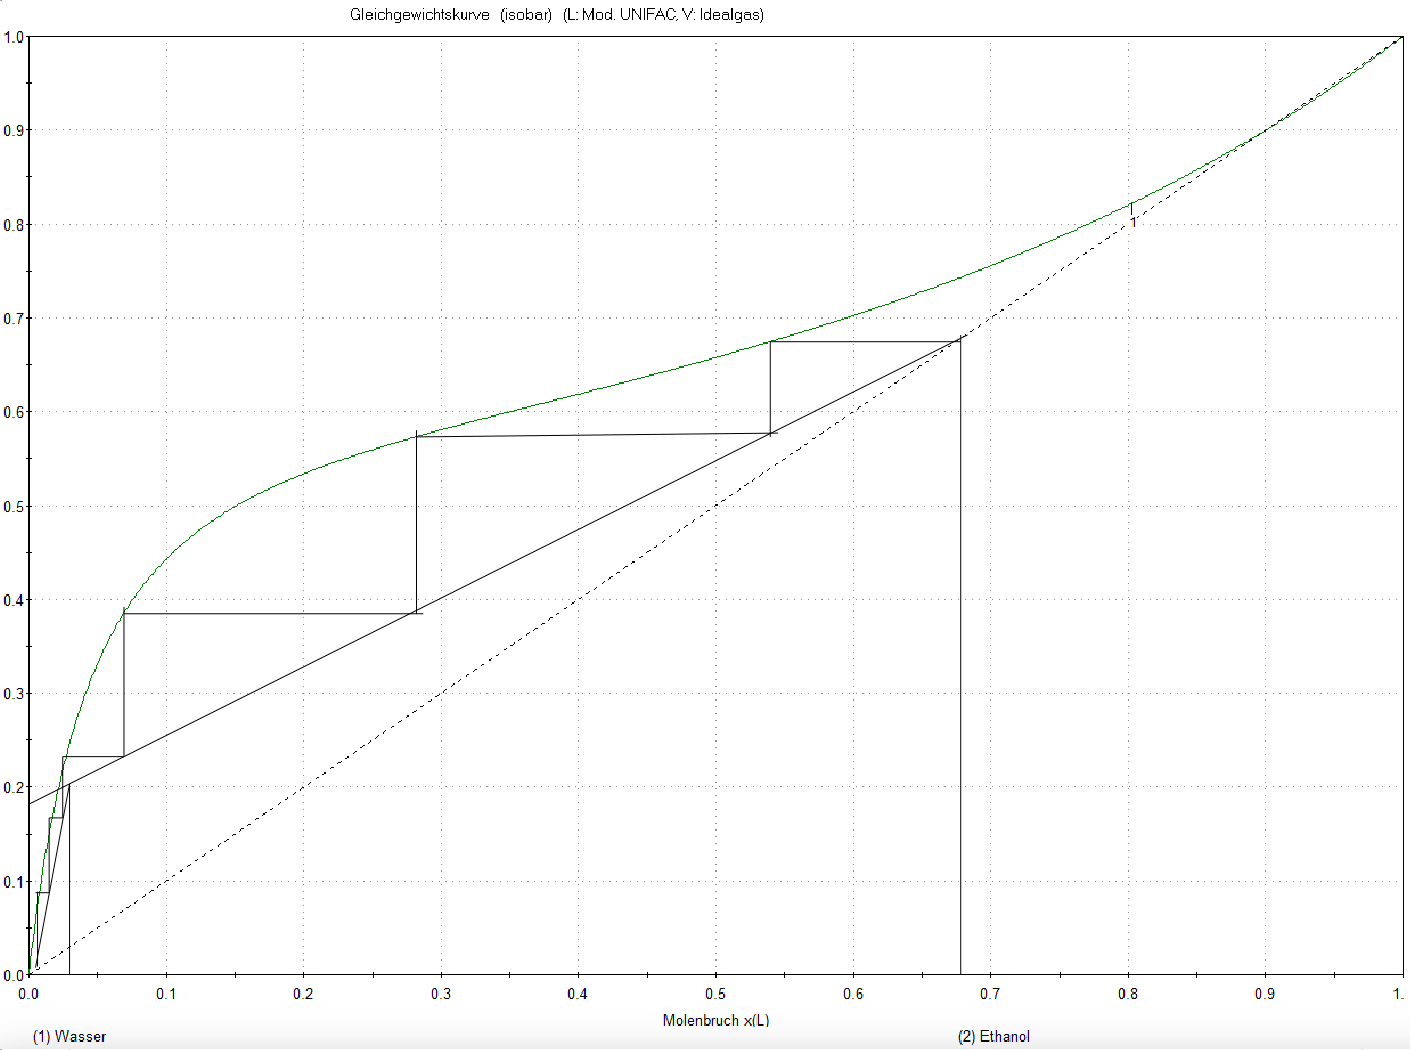
\includegraphics[width=0.85\linewidth]{img/McCabe}
	\caption{Das Gleichgewichtsdiagramm des Versuch 1 mit der resultierenden Stufenkonstruktion - von Hand}
	\label{fig:McCabe}
\end{figure}
\FloatBarrier
\begin{figure}[h!]
	\centering
	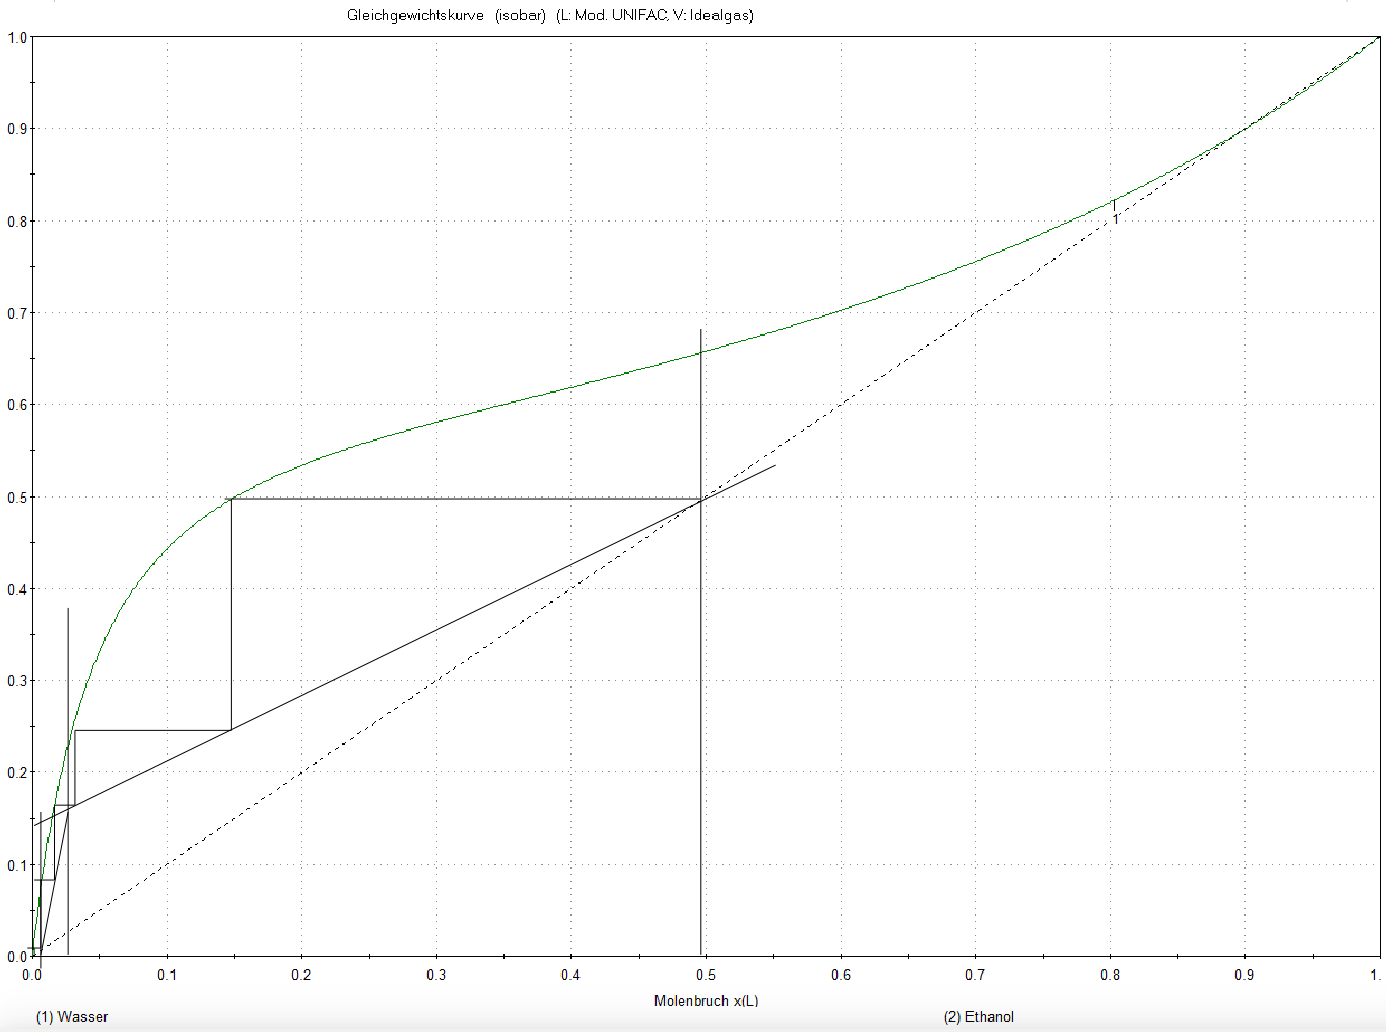
\includegraphics[width=0.85\linewidth]{img/McCabe2(5Stufen)}
	\caption{Das Gleichgewichtsdiagramm des Versuch 2 mit der resultierenden Stufenkonstruktion - von Hand}
	\label{fig:McCabe2}
\end{figure}
\FloatBarrier

\begin{figure}[h!]
	\centering
	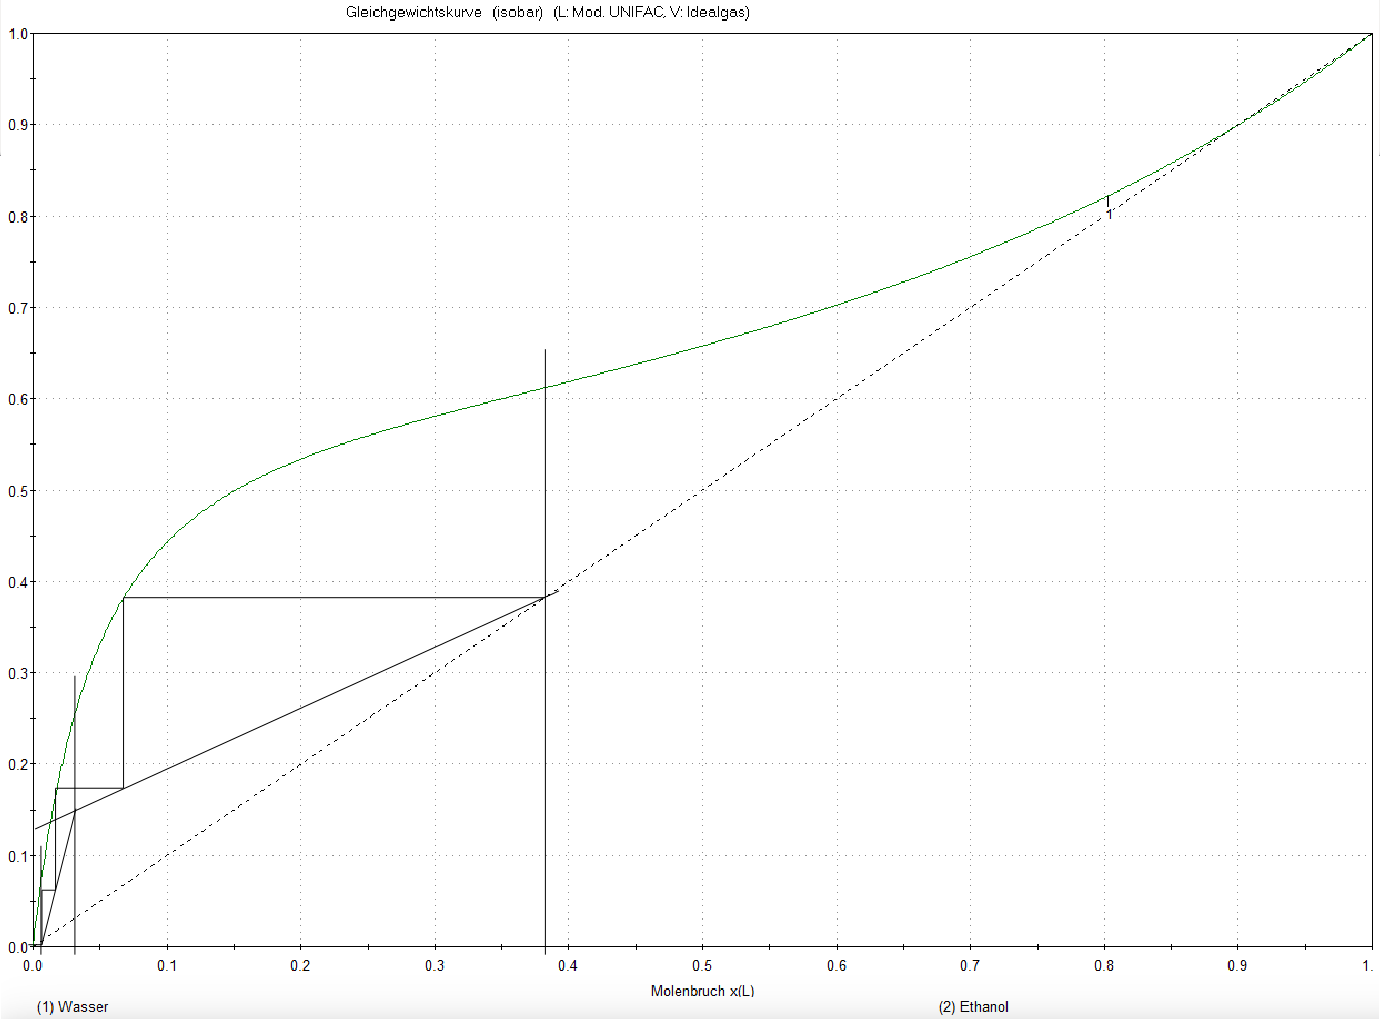
\includegraphics[width=0.85\linewidth]{img/McCabe3(4Stufen)}
	\caption{Das Gleichgewichtsdiagramm des Versuch 3 mit der resultierenden Stufenkonstruktion - von Hand}
	\label{fig:McCabe3}
\end{figure}
\FloatBarrier

\begin{figure}[h!]
	\centering
	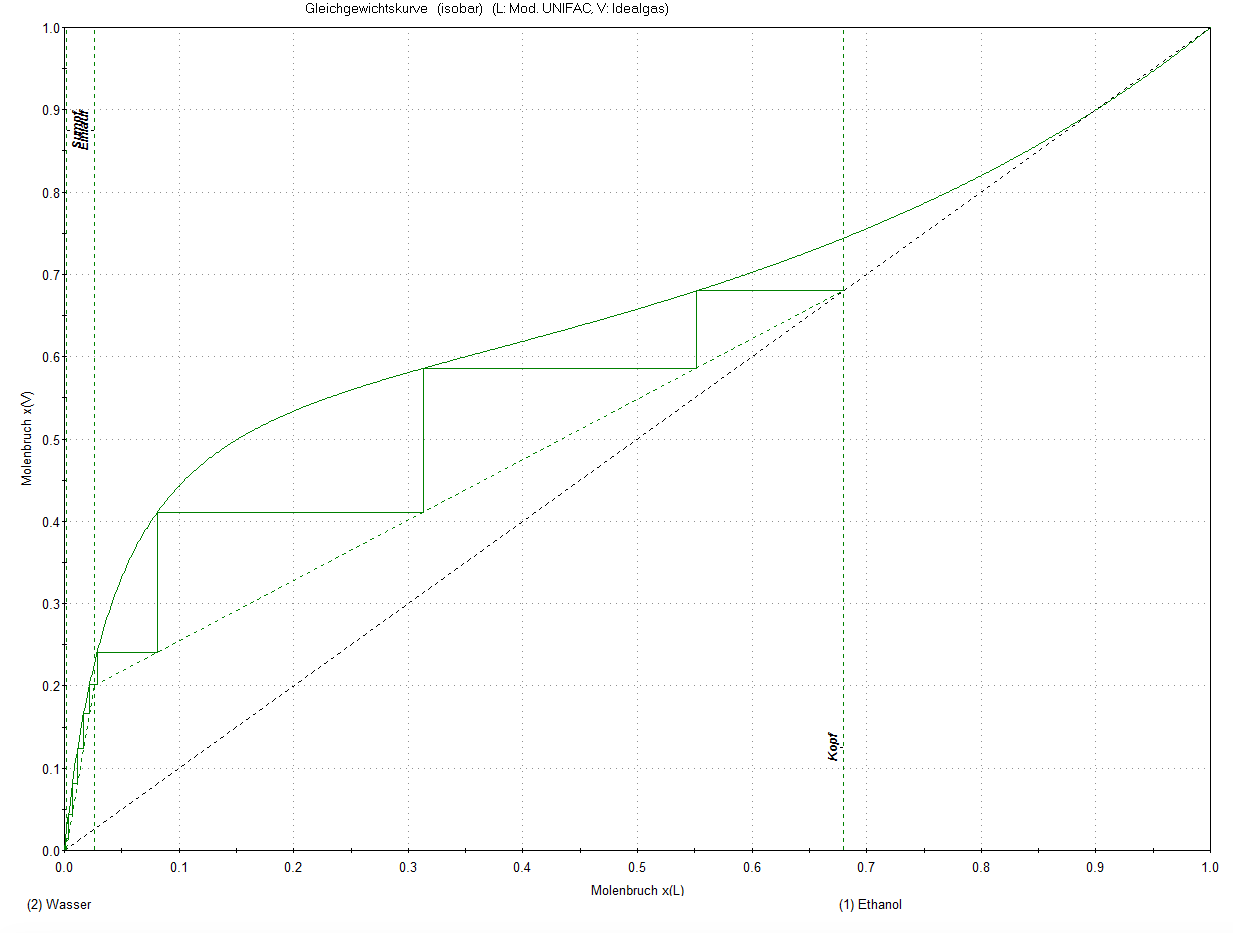
\includegraphics[width=0.85\linewidth]{img/VLE-MC-1}
	\caption{Das Gleichgewichtsdiagramm des Versuch 1 mit der resultierenden Stufenkonstruktion - automatisch}
	\label{fig:versuchsaufbau-ebull}
\end{figure}
\FloatBarrier
\begin{figure}[h!]
	\centering
	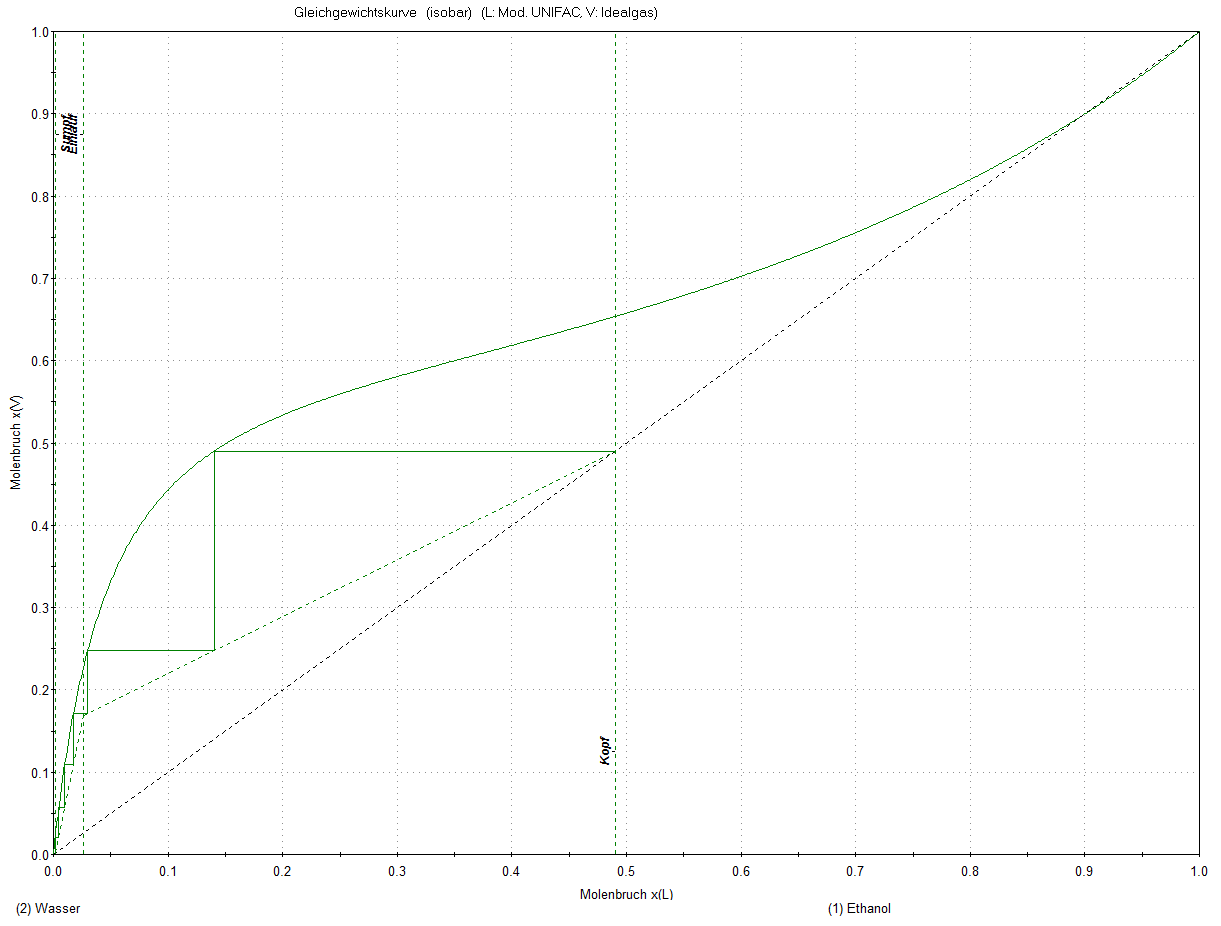
\includegraphics[width=0.85\linewidth]{img/VLE-Mc-2}
	\caption{Das Gleichgewichtsdiagramm des Versuch 2 mit der resultierenden Stufenkonstruktion - automatisch}
	\label{fig:versuchsaufbau-ebull}
\end{figure}
\FloatBarrier
\begin{figure}[h!]
	\centering
	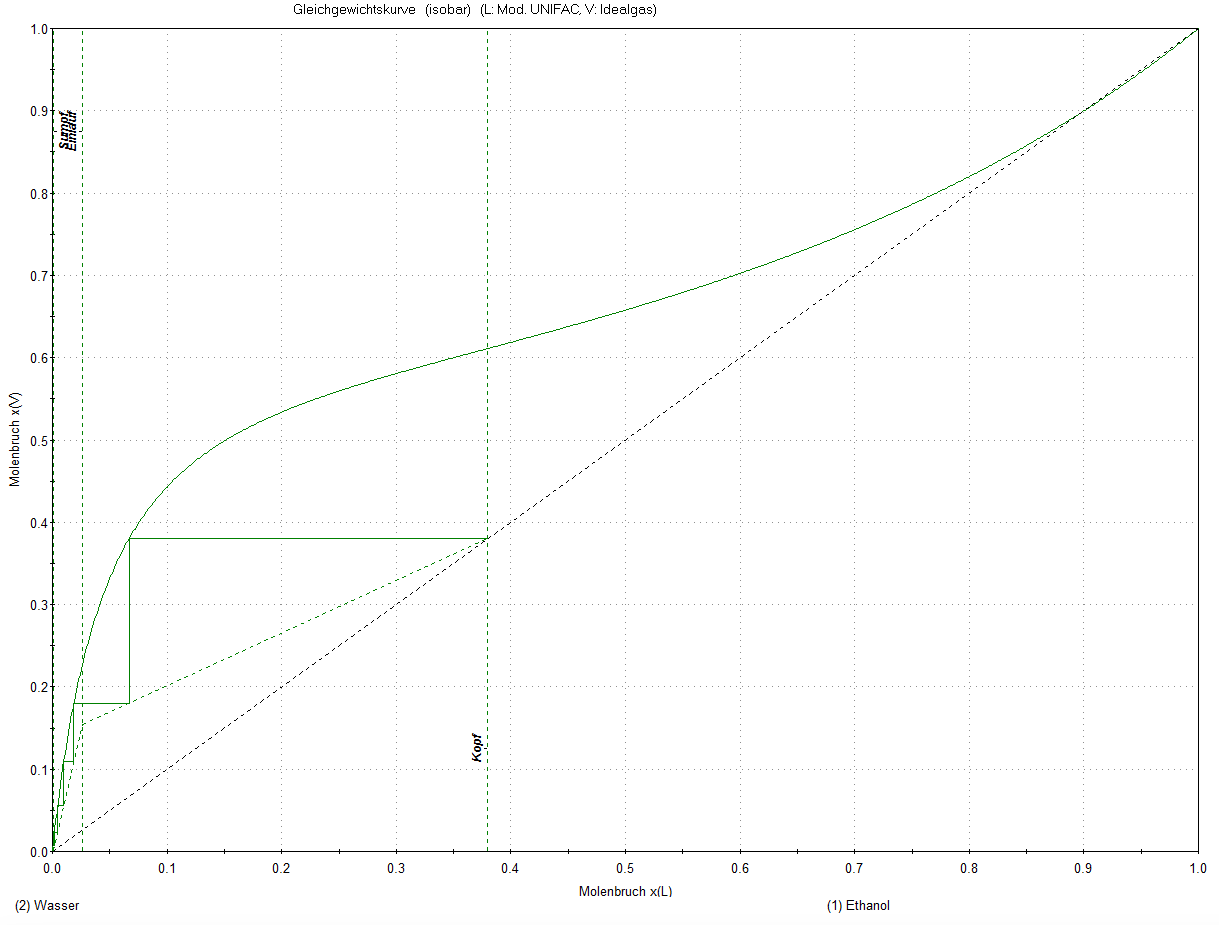
\includegraphics[width=0.85\linewidth]{img/VLE-Mc-3}
	\caption{Das Gleichgewichtsdiagramm des Versuch 3 mit der resultierenden Stufenkonstruktion - automatisch}
	\label{fig:versuchsaufbau-ebull}
\end{figure}
\FloatBarrier




\subsection{Energiebilanz}
Um in die Gleichung \eqref{gl:energiebilanzKOLONNE} als Energiebilanz einsetzen zu können, müssen zuerst die Enthalpien der Ströme berechnet werden. Für diese wiederum ist die spezifische Wärmekapazität erforderlich. Außerdem muss die Kühl und Heizleistung bekannt sein. Die Berechnungen sind in den nachfolgenden Abschnitten detailliert aufgeführt. Die Gleichung \eqref{gl:Energie-eingesetzt} enthält die eingesetzten Zwischenergebnisse. Durch diese Energiebilanz lässt sich die Verlustwärme berechnen. Diese beträgt im ersten Versuch \SI{637,5}{\watt}.
\begin{flalign}\label{gl:Energie-eingesetzt}
\dot{H}_F+Q_{Heiz}&=\dot{H}_K+\dot{H}_S+Q_{Kondensator}+Q_{Verlust}\\
	\SI{108,29}{\watt}+\SI{1229,36}{\watt}&=\SI{21,66}{\watt}+\SI{475,94}{\watt}+\SI{202,55}{\watt}+Q_{Verlust}\\
	Q_{Verlust}&=\underline{\SI{637,5}{\watt}}
\end{flalign}

\subsubsection{Wärmekapazitäten}
Die Wärmekapazitäten der Mischungen, werden durch Wichtung der Wärmekapazitäten der Reinstoffe, bei der gemessenen Temperatur, mit den Molenbrüchen, nach Gleichung \eqref{gl:cp} berechnet. Die Wärmekapazität der Reinstoffe ist durch dir Regressionsgleichung \eqref{gl:regCP} und die tabellierten Konstanten A, B, C, D und E gegeben.
\begin{equation}\label{gl:regCP}
	cp\,\, [\SI{}{\joule\per\kilo\mole\per\kelvin}]=A+B*T+C*T^2+D*T^3+E*T^4
\end{equation}
\begin{flalign}\label{gl:cp}
	\bar{c_p}(K)&=x_1*c_{p1}+x_2*c_{p2}\\
	&=0,68*\SI{138673}{\joule\per\kilo\mole\per\kelvin}+(1-0,68)*\SI{75569}{\joule\per\kilo\mole\per\kelvin}\\
	&=\underline{\SI{118481,84}{\joule\per\kilo\mole\per\kelvin}}
\end{flalign}

\subsubsection{Enthalpien der Ströme}

\begin{flalign}
	\dot{H}&=\dot{n}*cp*\Delta T\\
	\dot{H}_K&=\dot{n}_K*c_{pK}*\Delta T_K\\
	&=\SI{8,34}{\mole\per\hour}*\SI{118481,84}{\joule\per\kilo\mole\per\kelvin}*\SI{78,9}{\kelvin}\\
	&=\underline{\SI{21,66}{\watt}}\\%===================
	\dot{H}_F&=\dot{n}_F*c_{pF}*\Delta T_F\\
	&=\SI{236,995}{\mole\per\hour}*\SI{76386,75}{\joule\per\kilo\mole\per\kelvin}*\SI{21,65}{\kelvin}\\
	&=\underline{\SI{108,29}{\watt}}\\
		\dot{H}_S&=\dot{n}_S*c_{pS}*\Delta T_S\\
		&=\SI{227,27}{\mole\per\hour}*\SI{76112,46}{\joule\per\kilo\mole\per\kelvin}*\SI{99,05}{\kelvin}\\
		&=\underline{\SI{475,94}{\watt}}\\
\end{flalign}
\subsubsection{Kühlleistung}

\begin{flalign}
	\dot{Q}&=\dot{m}*c_p*\Delta T\\
	&=(\rho*\dot{V})*c_p*(T_\omega-T_\alpha)\\
	&=(\SI{999,38}{\kilogram\per\cubic\meter}*\SI{28,25e-3}{\cubic\meter\per\hour})*\SI{4200}{\joule\per\kilogram\per\kelvin}*(\SI{19,45}{\degreeCelsius}-\SI{13,3}{\degreeCelsius})*\si{\kelvin}\\
	&=\underline{\SI{202,55}{\watt}}
\end{flalign}
\subsubsection{Berechnung der Heizleistung}

Die Berechnung der Heizleistung in Watt beruht auf der verbrauchten Energie über einen gewissen Zeitraum. Definitionsgemäß kann daher die Heizleistung entsprechend der nachfolgenden Gleichung \eqref{gl:Qheizung} berechnet werden.

\begin{flalign}\label{gl:Qheizung}
\dot{Q}_{Heizung}&=\frac{Q_{Heizung}[W*h]}{t[s]/3600}\\
&=\frac{\SI{358,3}{\watt\hour}}{\SI{1049}{\second}/3600}\\
&=\underline{\SI{1229,36}{\watt}}
\end{flalign}

\newpage
\section{Diskussion}
\label{sec:diskussion}

Die Zahl der theoretischen Trennstufen aus der Stufenkonstruktion im McCabe-Thiele-Diagramm nimmt mit sinkender Kopfproduktreinheit ab. Wo für den Versuch 1 noch 6 Stufen konstruiert wurden, waren für den Versuch 2 nur noch 5 und für den Versuch noch 4 Stufen nötig. Natürlich blieb die Bodenzahl in der Versuchskolonne gleich. Die wirkliche Anzahl der Böden liegt immer weit über der theoretischen Zahl.

Aus den Berechnungen geht hervor, dass der Kopfproduktstrom bei sinkendem Rücklaufverhältnis ansteigt. Mit dem Rücklaufverhältnis sinkt aber auch die Konzentration an Leichtsieder im Produkt.

Der Vergleich der selbst berechneten Werte mit denen aus dem Programm VLE in Tabelle \ref{tab:Vergleich} ergibt, dass sich die Ergebnisse im großen und ganzen sehr ähneln. Die größten Abweichungen treten bei der Konstruktion des Mc-Cabe-Thiele Diagramms auf. Hier wurde eine theoretische Stufenzahl von 6, anstelle der 10 von VLE ermittelt. Das Ergebnis des Computerprogramms ist deutlich vertrauenswürdiger, da dabei die Lösung numerisch erfolgte. Die zeichnerische Lösung birgt durch die Ungenauigkeiten der Skalen ein hohes Potential für Abweichungen. Außerdem fällt auf, dass die Temperaturen am Kolonnenkopf um einige Kelvin höher sind als es durch das Programm prognostiziert wurde.

Der berechnete Wärmeverlust entspricht mit den in Gleichung \eqref{gl:Energie-eingesetzt} berechneten \SI{637,5}{\watt} 52\% der Heizleistung. Dies ist aufgrund der vielen un-isolierten Bereiche an der Kolonne plausibel. Die Korrektur des Rücklaufverhältnisses war in den gegebenen Werten bereits erfolgt. Das Ausgleichen der Stoffbilanz mittels des \emph{solver}, beruht auf der Annahme, dass die Messung des Kopfproduktvolumenstromes fehlerfrei ist.

\begin{table}[h!]
	\centering
	\caption{Vergleich der Ergebnisse aus händischer Berechnung zu den Ergebnissen des Programms VLE}
	\label{tab:Vergleich}
	\resizebox{16cm}{!}{
	\begin{tabular}{|c|c|c|c|c|c|}
		\hline
		Versuch Nr. &Rücklaufverhältnis &$x_{1K}$ &McCabe-Thiele Stufenzahl & $\vartheta$(Sumpf)[\si{\degreeCelsius}] &$\vartheta$(Kopf) [\si{\degreeCelsius}] \\
		\hline
			\multicolumn{6}{|c|}{gemessene und durch VLE berechnete Werte}      \\
		\hline
		1        & 2,76 & 0,68 & 10 & 99,64 & 78,71 \\
		2        & 2,26 & 0,49 & 6  & 99,48 & 79,89 \\
		3        & 1,76 & 0,38 & 5  & 99,41 & 80,80 \\
		\hline
		\multicolumn{6}{|c|}{gemessene und händisch bestimmte Werte}      \\
		\hline
		1        & 2,76 & 0,68 & 6  & 99,05 & 78,9  \\
		2        & 2,26 & 0,49 & 5  & 98,8  & 82,25 \\
		3        & 1,76 & 0,38 & 4  & 98,8  & 85 \\
		\hline
		
	\end{tabular}
	}
\end{table}
\FloatBarrier
\vspace*{-2.5mm}
%Tabelle Ende
Das Konzentrationsprofil in Ober- und Untersäule lässt sich ebenfalls aus den Gleichgewichtsdiagrammen ableiten. Dazu wird Anzahl und Form der Stufen links und rechts von der Feedkonzentration betrachtet. Es ergibt sich, dass die Konzentrationssprünge in der Obersäule, in diesem Experiment, immer größer sind als die in der Untersäule. Eine hohe Reinheit des Kopfprodukts und kleine Rücklaufverhältnisse bewirken mehr Stufen in der Obersäule, während sehr geringe Leichtsiederkonzentrationen in Feed und Sumpf besonders für eine hohe Stufenzahl der Untersäule verantwortlich sind. Die Konzentrationsprünge zwischen den Stufen sind in der Obersäule besonders groß. Das ist schon an der Gleichgewichtskurve zu erkennen. Je weiter sich diese von der Diagonalen weg wölbt, desto besser lässt sich ein Gemisch destillieren/ rektifizieren. Ein wirkliches Konzentrationsprofil lässt sich aus den gegebenen Daten jedoch nicht ableiten. Dazu wären die Temperaturen auf den einzelnen Böden nötig, um aus den Siedepunkten die genaue Zusammensetzung auf den einzelnen Glockenböden abzuleiten.




\section{Fehlerbetrachtung}
\label{sec:fehler}

Alle Messonden sind Fehlerbehaftet. Die digitale Kontrollwarte am PC verhindert einige Ablesefehler. Selbige könnten aber beim ablesen der Volumina trotzdem aufgetreten sein. Die Wärmekapazität wurde als Reienentwicklung in die Gleichungen einbezogen. Dieses Verfahren beruht auf einer Annäherung an den realen Verlauf dieser Größe. Die Regressionsgleichung vierten Grades ist als sehr genau einzustufen und wird daher nicht angezweifelt. Ebenso ist die Dichtemessung mit dem sehr präzisen Messgerät als praktisch fehlerfrei zu sehen.

Einige Berechnungen wurden von Hand gemacht. Im laufe der Auswertung könnten sich Übertragungsfehler eingeschlichen haben. Es ist sehr auffällig, dass die zeichnerische Bestimmung der Stufenzahl im McCabe-Thiele-Diagramm sehr Fehleranfällig ist. Das Ablesen und eintragen in an den Koordinatenachsen basiert auf dem Abschätzen von Zahlenwerten zwischen der groben einteilung. besonders am unteren Ende, wo die Konzentration von Feed und Sumpf sehr nah beieinander liegen, ist eine ausreichend genaue Eintragung unmöglich. Daher sind die Ergebnisse des Computerprogramms VLE als richtig anzunehmen.


Das Ausgleichen der Stoffbilanz mittels des \emph{solver}, beruht auf der Annahme, dass die Messung des Kopfproduktvolumenstromes fehlerfrei ist. Da dies keinesfalls sein kann, ist die Massenbilanz und darauf aufbauende Energiebilanz mit dem nötigen Abstand zu betrachten.

Die Beispielrechnungen wurden zum Teil Händisch ausgeführt, weswegen die Ergebnisse durch Rundungsfehler etwas von den Ergebnissen aus der Tabellenkalkulation abweichen können.

\section*{Anhang}
\addcontentsline{toc}{section}{Anhang}
\label{sec:anhang}
 
:\begin{table}[h!]
	\centering
	\caption{Gegebene Daten zum Versuch (Datensatz J)}
	\label{tab:Einwaagen}
	\resizebox{12.6cm}{!}{
		\begin{tabular}{|c|c|c|c|c|}
			\hline
\textbf{Größe}	& \textbf{Einheit}  & \textbf{Versuch 1} & \textbf{Versuch 2} & \textbf{Versuch 3} \\
	\hline
			$\rho_K$ & [kg/m3] & 832,3  & 867& 890,3\\
				$\rho_F$ & [kg/m3] & 989,48& 989,48  & 989,48\\
				$\rho_S$ & [kg/m3] & 997,67  & 997,7 & 997,9\\
			&  &                    & &                    \\
			$V_K$ & [L] & 0,1 & 0,1& 0,1\\
			$t_K$  &     & 00:16:08  & 00:15:27           & 00:12:40  \\
		$t_K$  & [s]  & 968  & 927                & 760  \\
		$\dot{V}_K$ & [L/h] & 0,372 & 0,388 & 0,474\\
			$\dot{V}_F$ & [L/h]   & 4,20 & 4,76 & 4,03  \\
			&   &   &   &   \\
			$\vartheta _K$    & [\si{\degreeCelsius}] & 78,9  & 82,25 & 85                 \\
			$\vartheta _F$& [\si{\degreeCelsius}] & 21,65  & 20,1 & 20,3  \\
			$\vartheta _S$                             & [\si{\degreeCelsius}]                    & 99,05              & 98,8               & 98,8               \\
			&                             &                    &                    &                    \\
			Kühler $\alpha$                      & [\si{\degreeCelsius}]                   & 13,3               & 12,8               & 12,5               \\
			Kühler $\omega$                     & [\si{\degreeCelsius}]                    & 19,45              & 18,95              & 18,25              \\
			$\dot{V}$  kühler                       & [L/h]                   & 28,25              & 28,5               & 28,45              \\
			&                             &                    &                    &                    \\
			$\dot{Q}$ Heizung $\alpha$                     & [Wh]                    & 1676,7             & 2330,1             & 2950,4             \\
		$\dot{Q}$  Heizung $\omega$                    & [Wh]                    & 2035               & 2731,2             & 3297,9             \\
			&                             &                    &                    &                    \\
			Startzeit                      &                             & 09:46:19           & 10:18:11           & 10:48:26           \\
			Endzeit                        &                             & 10:03:48           & 10:37:45           & 11:05:24           \\
			$\Delta t$ Heizung                      &                             & 00:17:29           & 00:19:34           & 00:16:58           \\
			$\Delta t$ Heizung                       & [s]                     & 1049               & 1174               & 1018               \\
			&                             &                    &                    &                    \\
			 $\dot{Q}$ Verlust  &  [W] &   \SI{637,5}{}                 &                    &                    \\
			&                             &                    &                    &                    \\
			t Rücklauf,Theorie              & [s]                     & 12                 & 10                 & 8                  \\
			t Entnahme,Theorie              & [s]                     & 3                  & 3                  & 3                  \\
			
			t Totzeit                       & [s]                     & 0,99               & 0,99               & 0,99               \\
			t Rücklauf,Praxis               & [s]                     & 11,01              & 9,01               & 7,01               \\
			t Entnahme,Praxis               & [s]                     & 3,99               & 3,99               & 3,99              \\
			\hline
			
		\end{tabular}
	}
\end{table}
\FloatBarrier
\vspace*{-2.5mm}
%Tabelle Ende
 
 :\begin{table}[h!]
 	\centering
 	\caption{Berechnungsergebnisse aus den Tabellenkalkulationsprogramm \emph{LibreOffice Calc} entsprechend der Formeln aus den obigen Beispielrechnungen}
 	\label{tab:Einwaagen}
 	\resizebox{12.6cm}{!}{
 		\begin{tabular}{|c|c|c|c|c|}
 				\hline
 				\textbf{Größe}	& \textbf{Einheit}  & \textbf{Versuch 1} & \textbf{Versuch 2} & \textbf{Versuch 3} \\
 				\hline
 		
 			$w_{1K} $            & & 0,845      & 0,707      & 0,608      \\
 			$w_{1F} $             & & 0,065      & 0,065      & 0,065      \\
 			$w_{1S} $              & & 0,004      & 0,004      & 0,002      \\
 			 & & & & \\
 			$x_{1K} $               & & 0,680      & 0,486      & 0,377      \\
			$x_{1F} $                & & 0,026      & 0,026      & 0,026      \\
 			$x_{1S} $                 & & 0,002      & 0,002      & 0,001      \\
 & & & & \\
	 		$\dot{n}_{1K}$      &[mol/h] & 5,67       & 5,17       & 5,56       \\
 			$\dot{n}_{1F}$     &[mol/h] & 5,86       & 6,64       & 5,62       \\
 & & & & \\
 			$\dot{n}_K$ original                        & [mol/h]& 8,34       & 10,64      & 14,74      \\
 			$\dot{n}_F$ original                 &[mol/h] & 221,31     & 250,98     & 212,42     \\
 			$\dot{n}_F$ aus solver              &[mol/h] & 235,60     & 214,57     & 223,46     \\
 			$\dot{n}_S$ aus solver              & [mol/h]& 227,27     & 203,93     & 208,72     \\
 & & & & \\
 			Delta T$_K$             & [K]& 78,9       & 82,25      & 85         \\
 			Delta T$_F$             &[K] & 21,65      & 20,1       & 20,3       \\
 			Delta T$_S$             &[K] & 99,05      & 98,8       & 98,8       \\
 			& & & & \\
 			$\Delta$Q             & {[}Wh{]}& 358,3      & 401,1      & 347,5      \\
 
 			Q Heizung           & {[}W{]}& 1.229,63   & 1.229,95   & 1.228,88   \\
 			Qkühlung          &{[}W{]}   & 202,57     & 204,36     & 190,73     \\
 			\hline
 			mittlere cp  & &            &            &            \\
 			K                          &{[}J/kmol*K{]} & 118.481,84 & 107.250,74 & 100.858,51 \\
 			F                          &{[}J/kmol*K{]} & 76.386,75  & 76.402,66  & 76.400,73  \\
 			S                          & {[}J/kmol*K{]}& 76.112,46  & 76.099,33  & 76.053,60  \\
 		\hline
 			& &            &            &            \\
 			$\dot{H}_K$                         &[W] & 21,67      & 26,07      & 35,11      \\
 			$\dot{H}_F$                         &[W] & 101,67     & 107,06     & 91,51      \\
 			$\dot{H}_S$                         & [W]& 493,38     & 448,13     & 466,42     \\
 			& &            &            &            \\
 			$\dot{Q}$ Verlust           &[W] & 613,68     & 658,45     & 628,13      	\\
 			\hline
 				\end{tabular}
 	}
 \end{table}
 \FloatBarrier
 \vspace*{-2.5mm}
 %Tabelle Ende

%Praktikumsskript, Modul ………, Versuch …….., Prof. Musterprof. 
%DIN 12345, Jahr der Veröffentlichung 
%Link der Internetseite, Zugriffsdatum 
%Buchtitel, Autor, Verlag, Veröffentlichungsjahr 

%Literaturverzeichnis Bücher
\bibliography{Literatur}
\bibliographystyle{unsrtdin}
\addcontentsline{toc}{section}{Literaturverzeichnis}

%\chapter*{Eidesstattliche Erklärung}
\label{erklaerung}
Hiermit versichere ich, die vorliegende Seminararbeit selbstständig und nur unter Verwendung der von mir angegebenen Quellen und Hilfsmittel verfasst zu haben. Sowohl inhaltlich als auch wörtlich entnommene Inhalte wurden als solche kenntlich gemacht. Die Arbeit hat in dieser oder vergleichbarer Form noch keinem anderem Prüfungsgremium vorgelegen. \\
\\[1.5cm]
Datum:	\hrulefill\enspace Unterschrift: \hrulefill
\\[3.5cm]
\addcontentsline{toc}{chapter}{Selbstständigkeitserklärung}

\end{document}
